\documentclass[9pt]{beamer}

\usepackage[utf8]{inputenc}

\def\today{\ifcase\month\or
January\or February\or March\or April\or May\or June\or
July\or August\or September\or October\or November\or December\fi
\space \number\year
} % \today of the form "Month Year"

\usetheme[progressbar=frametitle,outer/numbering=none]{metropolis}
\usepackage{appendixnumberbeamer}

\usepackage[square, numbers, comma, sort&compress]{natbib} % Use the natbib reference package - read up on this to edit the reference style; if you want text (e.g. Smith et al., 2012) for the in-text references (instead of numbers), remove 'numbers' 
\bibliographystyle{apsrev4-1-etal} % Use the utphys, apsrev4-1, kp and more BibTeX style for formatting the Bibliography
\usepackage{notoccite}

\usepackage{tabu}

\usepackage{amsmath,amsfonts,amssymb,amscd,amsthm,xspace,mathtools}
\usepackage[centerlast,small,sc]{caption}
\graphicspath{{Figures/},{../Thesis/Figures/}} % Specifies the directory where pictures are stored

%%% FONTS
\usefonttheme{serif}
\newcommand\hmmax{0}
\newcommand\bmmax{0}
\usepackage{mathpazo}
\usepackage{bm}

\DeclareMathAlphabet{\mathpzc}{OT1}{pzc}{m}{it}
\DeclareSymbolFont{cmletters}{OT1}{cmr}{m}{n}
\DeclareMathSymbol{\Upsilon}{\mathalpha}{cmletters}{"7}

\usepackage[bbgreekl]{mathbbol}
\DeclareSymbolFontAlphabet{\mathbb}{AMSb}
\DeclareSymbolFontAlphabet{\mathbbl}{bbold}

\usepackage[mathscr]{euscript}

\newcommand{\lambdabar}{{\mkern 0.0mu\lambda\mkern -8.2mu\mathchar '26\mkern 2mu}}

\newcommand{\xdownarrow}[1]{%
	{\left\downarrow\vbox to #1{}\right.\kern-\nulldelimiterspace}
}
\newcommand{\xDownarrow}[1]{%
	{\left\Downarrow\vbox to #1{}\right.\kern-\nulldelimiterspace}
}


\newcommand{\dd}{\mathrm{d}}
\newcommand{\uu}[3][]{ {}_{#1} #2_{#3} }
\renewcommand{\Re}{\mathrm{Re}}
\renewcommand{\Im}{\mathrm{Im}}

\setbeamerfont{frametitle}{size=\Large,shape=\scshape}
\setbeamerfont{title page}{size=\Large,shape=\scshape}

%-------------------------------------------------------------------------------------



\title{\scshape\LARGE Aspects of superradiant scattering \\ off Kerr black holes}
%\subtitle{A modern beamer theme}
\date{November 2017}
\author{\textbf{José \textsc{Sá}} \hfill \textit{Supervisor:} João G. \textsc{Rosa} \\[0.15cm] \phantom{arg} \hfill \textit{Co-supervisor:} Orfeu \textsc{Bertolami} \\[0.4cm]}
\institute{Faculdade de Ciências da Universidade do Porto}
% \titlegraphic{\hfill\includegraphics[height=1.5cm]{logo.pdf}}



\begin{document}

\maketitle

% \begin{frame}{Table of contents}
%     \setbeamertemplate{section in toc}[sections numbered]
%     \tableofcontents[hideallsubsections]
% \end{frame}

\begin{frame}[fragile]{Outline}
    \begin{itemize}
        \large
        \setlength\itemsep{1.2em}
        \item What is superradiance ?
        \item Kerr black hole and the Penrose process
        \item Newman-Penrose formalism and the Teukolsky equation
        \item Analytical approximated solutions
        \item Numerical methods
        \item Scattering of planes waves 
        \item Conclusions and future work
    \end{itemize}
\end{frame}

{
    \usebackgroundtemplate{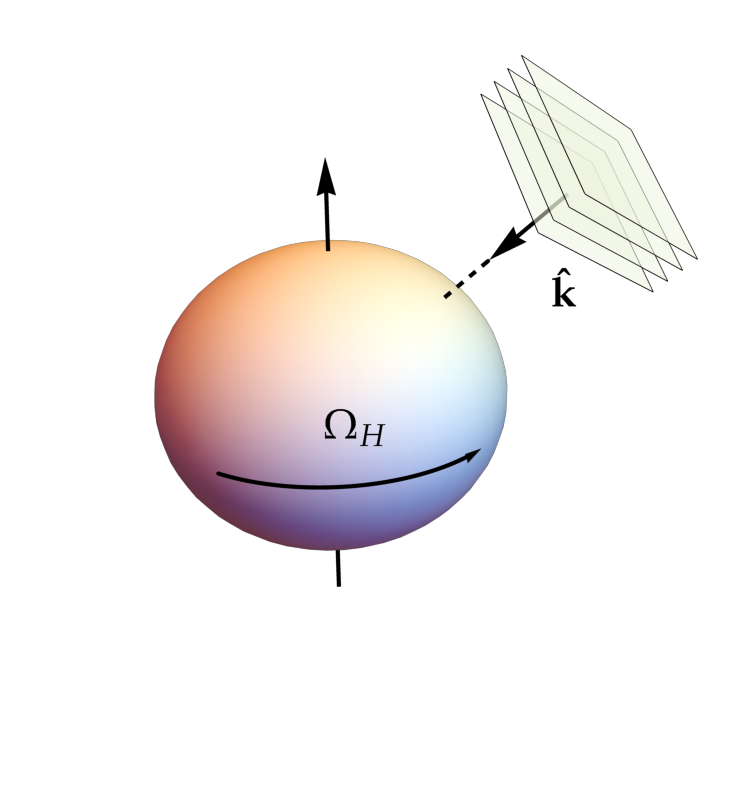
\includegraphics[scale=0.55,trim=-11cm 0 0 -3cm]{test.pdf}}
    \begin{frame}[fragile]{Introduction}

        \begin{columns}[T,onlytextwidth]        
            \column{0.5\textwidth}
        
                \metroset{block=fill}
        
                \begin{block}{Default}
                Block content.
                \end{block}
        
                \begin{alertblock}{Alert}
                Block content.
                \end{alertblock}
        
                \begin{exampleblock}{Example}
                Block content.
                \end{exampleblock}
        
        \end{columns}

    \end{frame}
}

\begin{frame}[fragile]{Kerr black hole}

    \vspace{0.15cm}

    \metroset{block=fill}
    \begin{block}{Boyer-Lindquist coordinates}
        \begin{align*}
            \begin{split}
                ds^2 = & \left(1 - \frac{2 M r}{\rho^2} \right) \dd t^2 + 2 a \sin^2\theta \frac{(r^2+a^2-\Delta)}{\rho^2} \dd t \dd \varphi \\
                &- \frac{(r^2+a^2)^2- \Delta a^2 \sin^2\theta}{\rho^2} \sin^2\theta \dd\varphi^2 - \frac{\rho^2}{\Delta} \dd r^2 - \rho^2 \dd \theta^2
            \end{split}
        \end{align*}
        \centering
        $\scriptstyle [\,\Delta=r^2 - 2 M r + a^2 ~,~~ \rho^2 = r^2 + a^2 \cos^2\theta\,]$
    \end{block}

    \begin{itemize}
        \setlength\itemsep{0.8em}
        \item BH angular momentum $J = a M \quad\left[ a=0 ~\Rightarrow \text{Schwarzschild} \right]$ 
        \item Killing vectors $\partial_t$ (stationary) and $\partial_\varphi$ (axisymmetric)
        \item Horizons at $g^{rr}=0 ~\Rightarrow~ \Delta=0 ~\Rightarrow~ r = r_{\pm} \equiv M \pm \sqrt{M^2-a^2}$ \\
        \emph{Cosmic censorship} conjecture $~\Rightarrow~$ $|a| \le M$
        
        \item Infinite redshift boundary $g_{tt}=0 ~\Rightarrow$ \alert{Ergoregion} $(g_{tt}<0)$
        $$r_+<r<r_\mathrm{ergo}(\theta) \equiv M + \sqrt{M^2 - a^2 \cos^2\theta}$$
    \end{itemize}
\end{frame}

\begin{frame}[fragile]{Penrose process}
    \begin{itemize}
        \setlength\itemsep{0.8em}
        \item Particle decays into two inside the ergoregion: $\bm{p} = \bm{p_1} + \bm{p_2}$
        \vspace{0.1cm}
        \begin{columns}[T,onlytextwidth]        
            \begin{column}{0.7\textwidth}
                \centering
                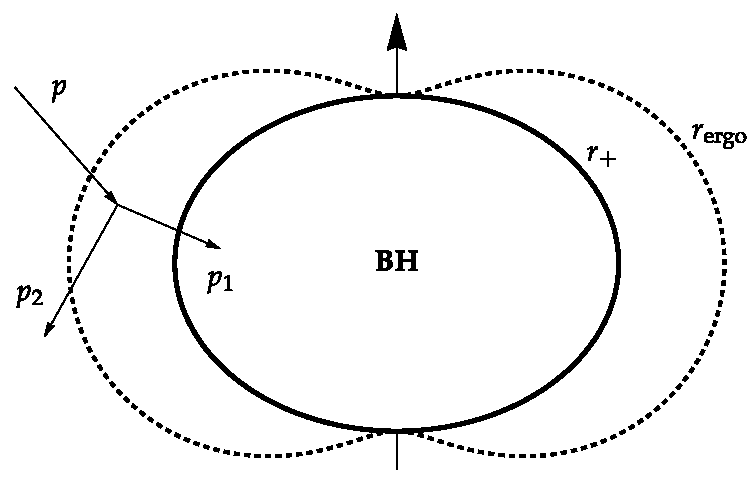
\includegraphics[scale=0.55,trim=0.3cm 0.3cm 0 0.3cm]{ergoPenrose.pdf}
            \end{column}
            \hfill
            \begin{column}{0.26\textwidth}
                \vspace*{0.5cm}
                \metroset{block=fill}
                \begin{block}{\small Killing horizon}
                    \footnotesize Hypersurface $r=r_{+}$ with normal null vector $$\bm{\xi} = \partial_t + \Omega_H \partial_\varphi \,\qquad$$ 
                    
                    Event horizon angular momentum:
                    $$\Omega_H = \frac{a}{2 M r_+} \qquad$$
                \end{block}
            \end{column}
        \end{columns}
        \vspace{0.3cm}
        \item We may have $E_1 = \bm{k} \cdot \bm{p_1} < 0 ~\Rightarrow E_2 = E + |E_1| > E $
        \item Local energy condition $\bm{\xi}\cdot\bm{p_1}>0$ at $r=r_{+} ~\Rightarrow E_1 - \Omega_H \, L_1 > 0$
        $$ \psi \sim e^{-i \omega t + i m \varphi} ~\Rightarrow~ \frac{\delta J}{\delta M} = \frac{\hbar m}{\hbar \omega} ~\Rightarrow~ \boxed{~\delta M < 0 ~\land~ \omega( \omega - \Omega_H \,m) < 0~} $$\\
        \hspace*{6.0cm}\alert{Energy extraction !}
    \end{itemize}
\end{frame}

\begin{frame}{Newman-Penrose formalism}    
    \begin{itemize}
        \setlength\itemsep{1.2em}
        \item EM perturbations $A^\mu \ll 1 ~\Rightarrow~ R_{\mu\nu} = \mathcal{O}(A^2)  ~\Rightarrow\text{fixed background} $

        \item Projection of tensors onto a tetrad frame of complex vectors
        $(\bm{\mathfrak{l}},\bm{\mathfrak{n}},\bm{\mathfrak{m}},\bar{\bm{\mathfrak{m}}})$
        %with $\bm{\mathfrak{l}}\cdot\bm{\mathfrak{m}} = \bm{\mathfrak{n}}\cdot\bm{\mathfrak{m}} = 0 ~,~~ \bm{\mathfrak{l}}\cdot\bm{\mathfrak{n}} = 1 ~,~~ \bm{\mathfrak{m}}\cdot\bar{\bm{\mathfrak{m}}} = -1$
        \begin{equation*}
            \underbrace{\mathbf{E} ~,~ \mathbf{B}}_\text{6 real components}
            \quad\longrightarrow\quad
            \boxed{
            \begin{aligned}
                \phi_0 &= F_{\mu\nu} \mathfrak{l}^\mu \mathfrak{m}^\nu \\
                \phi_1 &= \tfrac{1}{2} F_{\mu\nu} ( \mathfrak{l}^\mu \mathfrak{n}^\nu - \mathfrak{m}^\mu \bar{\mathfrak{m}}^\nu ) \\
                \phi_2 &= F_{\mu\nu} \bar{\mathfrak{m}}^\mu \mathfrak{n}^\nu 
            \end{aligned}
            }
            %\quad\text{and}\quad\text{c.c.} \Leftrightarrow (\bm{\mathfrak{m}}%\rightleftarrows \bar{\bm{\mathfrak{m}}})
        \end{equation*}
		
		\item \textbf{Kinnersley tetrad}
		\begin{alignat*}{3}
		\bm{\mathfrak{l}} &= \frac{1}{\Delta} \Big( r^2+a^2, \,\Delta, \,0, \,a \Big)&& \qquad\bm{\mathfrak{\texttt{}m}} = \frac{1}{\sqrt{2} \bar{\rho}} \Big( i \,a \sin\theta, \,0, \,1, \,i \csc\theta \Big) \\
		\bm{\mathfrak{n}} &= \frac{1}{2 \rho^2} \Big( r^2+a^2, -\Delta, \,0, \,a \Big) && \qquad\bar{\bm{\mathfrak{m}}} = \bm{\mathfrak{m}}^*
		\hspace*{1.6cm} {\scriptstyle [\,\bar{\rho} = r + i \,a \cos\theta \,]}
		\end{alignat*}
	
        Tetrad particularly suitable for the study of incoming and outgoing radiation $ \Rightarrow $ \alert{equations decouple}
        \begin{align*}
            \bm{\mathfrak{l}} \sim \partial_t + \partial_r \quad\qquad
            2\,\bm{\mathfrak{n}} \sim \partial_t - \partial_r
        \end{align*}

        % \item Equations written using tetrad derivatives $(\mathbbl{D}, \mathbbl{\Delta}, \bbdelta, \bar{\bbdelta})$ and spin connection $\gamma_{cab} = (e_c)^\mu (e_b){}^\nu \nabla_\nu (e_a)_{\mu} ~\Rightarrow~ \lambda, \pi, \tau, \varrho, \varepsilon, \sigma,\kappa, \gamma ,\mu, \nu, \alpha,\beta$
        % \begin{equation*}
        %     \begin{aligned}[c]
        %         \nabla_\mu F^{\mu\nu} &= 0 \\
        %         \nabla_{[\mu} F_{\nu\rho]} &= 0
        %     \end{aligned}
        %     \quad\longrightarrow~\left\{~~
        %     \begin{aligned}[c]
        %         \mathbbl{D} \phi_2 - \bar{\bbdelta} \phi_1 &= -\lambda \phi_0 + 2 \pi \phi_1 + (\varrho - 2 \varepsilon) \phi_2 \\
        %         \mathbbl{\Delta} \phi_1 - \bbdelta \phi_2 &= \nu \phi_0 - 2 \mu \phi_1 + (2\beta-\tau) \phi_2 \\
        %         \mathbbl{D} \phi_1 - \bar{\bbdelta} \phi_0 &= (\pi - 2 \alpha) \phi_0 + 2 \varrho \phi_1 - \kappa \phi_2 \\
        %         \mathbbl{\Delta} \phi_0 - \bbdelta \phi_1 &= (2 \gamma - \mu) \phi_0 - 2 \tau \phi_1 + \sigma \phi_2
        %     \end{aligned}
        %     \right.
        % \end{equation*}
    \end{itemize}

\end{frame}

\begin{frame}[fragile]{Newman-Penrose formalism}
    $\nabla_\mu F^{\mu\nu} = 0 ~,~ \nabla_{[\mu} F_{\nu\rho]} = 0  ~\longrightarrow~$ 4 complex first-order coupled equations
    $$\hspace{1.0cm}\xDownarrow{0.8cm} \quad\mathscr{D}_n \,, \mathscr{D}_n^\dagger = \partial_r \mp i K / \Delta + 2n(r-M)/\Delta \qquad 
    \mathscr{L}_n \,, \mathscr{L}_n^\dagger = \partial_\theta \mp Q + n \cot\theta $$
	Eliminate $\phi_1$ and rewrite $\Phi_0 = \phi_0 ~,~ \Phi_2 = 2 (\bar{\rho}^*)^2 \,\phi_2$ :
	\begin{itemize}
		\item 2 equations with eigenvalue $\lambdabar$
		\begin{align*}
			\left[ \Delta \mathscr{D}_1 \mathscr{D}^\dagger_1 + \mathscr{L}^\dagger_0 \mathscr{L}_1 + 2 i \omega (r+i a \cos\theta) \right] \Phi_0 &= 0 \\
			\left[ \Delta \mathscr{D}^\dagger_0 \mathscr{D}_0 + \mathscr{L}_0 \mathscr{L}^\dagger_1 - 2 i \omega (r+i a \cos\theta) \right] \Phi_2 &= 0
		\end{align*}
		
		\item 2 equations with relative normalization $\mathscr{B} = \sqrt{\lambdabar^2 - 4 a^2 \omega^2 + 4 a \omega m}$
		\begin{equation*}
		\begin{aligned}
			\mathscr{L}_0 \mathscr{L}_1 \Phi_0 &= \mathscr{D}_0 \mathscr{D}_0 \Phi_2 ~\\
			\mathscr{L}^\dagger_0 \mathscr{L}^\dagger_1 \Phi_2 &= \Delta \mathscr{D}^\dagger_0 \mathscr{D}^\dagger_0 \Delta \Phi_0
		\end{aligned}
%		~~\Rightarrow~
%		\begin{aligned}
%			( \mathscr{L}_0 \mathscr{L}_1 S_{+1} )/S_{-1} &= ( \Delta \mathscr{D}_0 \mathscr{D}_0 R_{-1})/(\Delta R_{+1}) = \mathscr{B} \\
%			( \mathscr{L}^\dagger_0 \mathscr{L}^\dagger_1 S_{-1} )/S_{+1} &= ( \Delta \mathscr{D}^\dagger_0 \mathscr{D}^\dagger_0 \Delta R_{+1} )/R_{-1} = \mathscr{B}
%		\end{aligned}
		\end{equation*}
	\end{itemize}
	\vfill
	Whats the form of the eigenvalue $\lambdabar$ ?

\end{frame}

\begin{frame}{Teukolsky equation}
	\begin{block}{General perturbation solution $\displaystyle 
			\quad\Rightarrow~ \Upsilon_s = \int\dd\omega \,\sum_{\ell,m} e^{-i\omega t + i m \varphi} \, {}_{s}S_{\ell m}(\theta)\, {}_{s}R_{\ell m}(r)$}
		\begin{itemize}
			\item Scalar $(s=0)$
			\item Electromagnetic $(s=\pm1)$ \hspace*{1cm}$\boxed{\Upsilon_{+1} = \phi_0 \qquad \Upsilon_{-1} = 2 (\bar{\rho}^*)^2 \phi_2 }$
			\item Gravitational $(s=\pm 2)$
		\end{itemize}
	\end{block}

	\begin{block}{Angular equation $\hfill\scriptstyle [\, z = \cos\theta ~,~ c = a \omega \,]$}
		\begin{center}
			$\displaystyle \frac{\dd}{\dd z} \left[ (1-z^2) \frac{\dd\, {}_{s}S_{\ell m}}{\dd z} \right] + \left[ (c z)^2 - 2 c s z  -\frac{(m + s z)^2}{1 - z^2} + s + {}_{s}\mathscr{A}_{\ell m} \right] {}_{s}S_{\ell m} = 0 $
		\end{center}
		\begin{itemize}
			\setlength\itemsep{1em}
			\item $c=0$ $~\Rightarrow$ Spherical symmetry (closed form) 
			\begin{center}
				$ e^{i m \varphi} \,{}_{s}S_{\ell m}(\theta) = {}_{s}Y_{\ell m}(\theta,\varphi)
				\hspace*{0.8cm}{}_{s}\mathscr{A}_{\ell m} = \ell(\ell+1)-s(s+1)$
			\end{center}
			\item $c\ne0$ $~\Rightarrow$ Series approximation or numerical methods (Leaver/Spectral)
			$${}_{s}\mathscr{A}_{\ell m} &= \ell(\ell+1) -s(s+1) - \frac{2 m s^2}{\ell(\ell+1)} c + \mathcal{O}(c^2)$$
		\end{itemize}
	\end{block}

\end{frame}


\begin{frame}{Teukolsky equation}
	
	\begin{block}{Radial equation $\quad \frac{1}{\Delta^s} \frac{\dd}{\dd r} \left( \Delta^{s+1} \frac{\dd\, {}_{s}R_{\ell m}}{\dd r} \right)
+ \left[ \frac{K^2 - 2 i s (r-M)K}{\Delta} + 4 i s \omega r -\lambda \right] {}_{s}R_{\ell m} = 0$}
		$$ \hspace*{2cm} {\color{orange}\Rightarrow} \left( \frac{\dd^2}{\dd r_{*}^2} + V_\mathrm{eff} \right) {}_{s}U_{\ell m} = 0 \hspace*{3cm} {\scriptstyle \left[~\frac{\dd r_*}{\dd r} = \frac{r^2+a^2}{\Delta}~\right] } $$
		where $\lambda = {}_{s}\mathscr{A}_{\ell m} - 2 m a \omega + a^2 \omega^2~$ and $~{}_{s}U_{\ell m}=\sqrt{\Delta^s (r^2 + a^2)} \,{}_{s}R_{\ell m}~$
		
		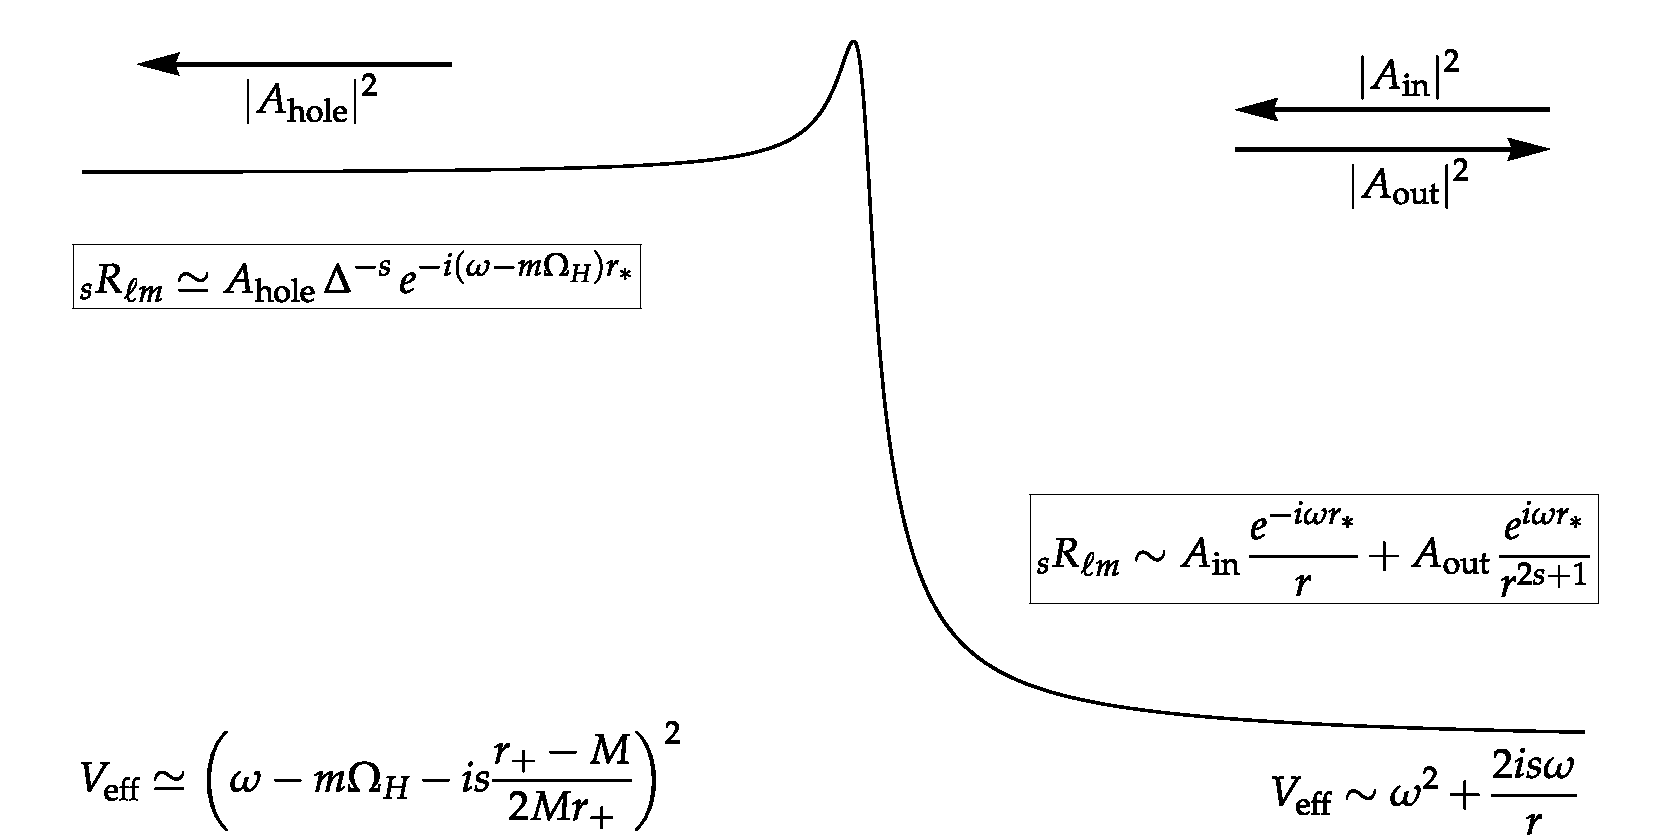
\includegraphics[scale=0.4]{Veff.pdf}
	\end{block}
	
\end{frame}


\begin{frame}{Analytical results}
	
	\begin{block}{Matching of coefficients}
		\begin{itemize}
			\setlength\itemsep{0.6em}
			\item Solving radial equation for $r - r_+ \gg r_+$ (far) and $r - r_+ \ll \omega^{-1}$ (near)
			
			\item Extend validity of the solutions to opposite regions and match dominant monomials of $x^{\ell-s}$ and $x^{-\ell-1-s}$ $~\Rightarrow~$ valid for modes $\bar{\omega}\equiv \omega r_+ \ll 1$
			\begin{center}
				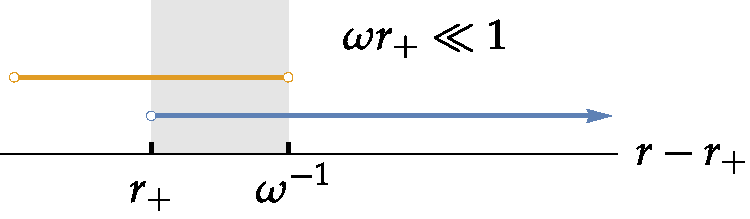
\includegraphics[scale=0.4]{validitySol}
			\end{center}	
		
			\item Obtain loss/gain factor $~\boxed{\displaystyle ~{}_{\pm 1}Z_{\ell m} = \frac{\dd E_\mathrm{out}}{\dd t}\bigg/\frac{\dd E_\mathrm{in}}{\dd t} - 1~}$
			\begin{align*}
				\uu[\pm1]{Z}{\ell m} \simeq  - 4 \bar{\omega} (\bar{\omega} - m \bar{\Omega}_H) \underbrace{(2-\tau)(2\bar{\omega} \tau)^{2\ell} \left[\frac{(\ell-1)! (\ell+1)!}{(2\ell)! (2\ell+1)!}\right]^2 \prod_{n=1}^{\ell} \left(n^2 + \frac{4 \varpi^2}{\tau^2} \right)}_\text{always $\ge 0$}
			\end{align*}
			
			\item Mode amplification $\uu[\pm1]{Z}{\ell m}>0 ~~{\color{orange}\Rightarrow}~ \omega (\omega - m \Omega_H) < 0$  
		\end{itemize}
		$\scriptstyle \hfill [~ x = (r-r_{+})/r_{+} ~,~ \tau = (r_{+}-r_{-})/r_{+} ~,~ \varpi = (2-\tau)(\bar{\omega} - m \bar{\Omega}_H) ~]$
	\end{block}
	
\end{frame}

\begin{frame}{Numerical methods}
	\begin{itemize}
		\setlength\itemsep{1em}

		\item Dependent variables $(\mathscr{J} = a/M, \,\bar{\omega}, \, \ell, \, m)$
		
		\item
		$\uu[\pm 1]{R}{\ell m} = (r_+)^{\mp 1} \, x^{ \mp 1 - i \varpi / \tau} f_{\pm}(x) \Rightarrow$ removes singular points of the eq.
		
		\item
		Integrate from $\epsilon\ll 1$ (stiffness) up to $x_\infty = 2\pi/\bar{\omega} \times 200$
		$$ f_{\pm}(\epsilon) = \sum_{n=0}^{N_H} \left(\frac{a_n}{a_0}\right)
		\,\epsilon^n ~~\Rightarrow~ f_{\pm}{}(\epsilon) \simeq 1 ~,~~ f_{\pm}{}'(\epsilon) \simeq 0$$
		
		\item
		Using conservation of energy $~\frac{\dd E_\mathrm{in}}{\dd t} - \frac{\dd E_\mathrm{out}}{\dd t} = \frac{\dd E_\mathrm{hole}}{\dd t}$
		\\[0.3cm]
		\begin{center}
			\tabulinesep=0.2em
			\begin{tabu}{@{\hskip 0.25cm}c@{\hskip 0.75cm}c@{\hskip 0.75cm}}
				\hline
				$\uu[\pm 1]{Z}{\ell m}$ & Solutions \\
				\hline\hline
				$\frac{\mathscr{B}^2 \tau^4 }{4 \varpi^2 (\tau^2 + 4 \varpi^2)} \left| \frac{f_{-}(x_\infty)}{f_{+}(x_\infty)} \right|^2 - 1$ & 
				$\phi_0$ and $\phi_2$ \\
				\hline
				$- \frac{\bar{\omega} \tau^2}{\varpi} \left|\frac{1}{f_{+}(x_\infty)}\right|^2$ &
				$\phi_0$ \\
				\hline
				$-1\bigg/\left( 1 + \frac{\mathscr{B}^2 \tau^2 \left|f_{-}(x_\infty)\right|^2}{4 \bar{\omega} \varpi(\tau^2 + 4 \varpi^2)} \right)$ & $\phi_2$ \\
				\hline
			\end{tabu}
		\end{center}
	\end{itemize}
	\vspace*{0.3cm}
	$\hfill\scriptstyle [~ \mathscr{B}^2 = ( \uu[-1]{\mathscr{A}}{\ell m} + a^2\omega^2 - 2 m a \omega )^2 - 4 a^2\omega^2 + 4 m a \omega ~]$
\end{frame}


\begin{frame}{Numerical methods}
	\begin{columns}
		\begin{column}{0.45\textwidth}
			\begin{itemize}
				\setlength\itemsep{1.5em}
				\item $\uu[s]{Z}{\ell m}(-\omega) = \uu[s]{Z}{\ell, -m}(\omega)$

				\item Maximum EM amplification:
				$$\sim \mathbf{4.4\%}$$
				for $\ell=m=1 ~,~  \omega M \simeq 0.436$

				\item Non-superradiant modes $$|\omega|\gg|m\Omega_h| ~\Rightarrow {}_{\pm 1}{Z}_{\ell m} \to 1 $$ (fully reflected)

				\item Superradiant modes
				$$ \text{increase } \ell ~\Rightarrow {}_{\pm 1}{Z}_{\ell m} \to 0 $$
				(potential centrifugal barrier)
			\end{itemize}
		\end{column}
		\begin{column}{0.55\textwidth}
			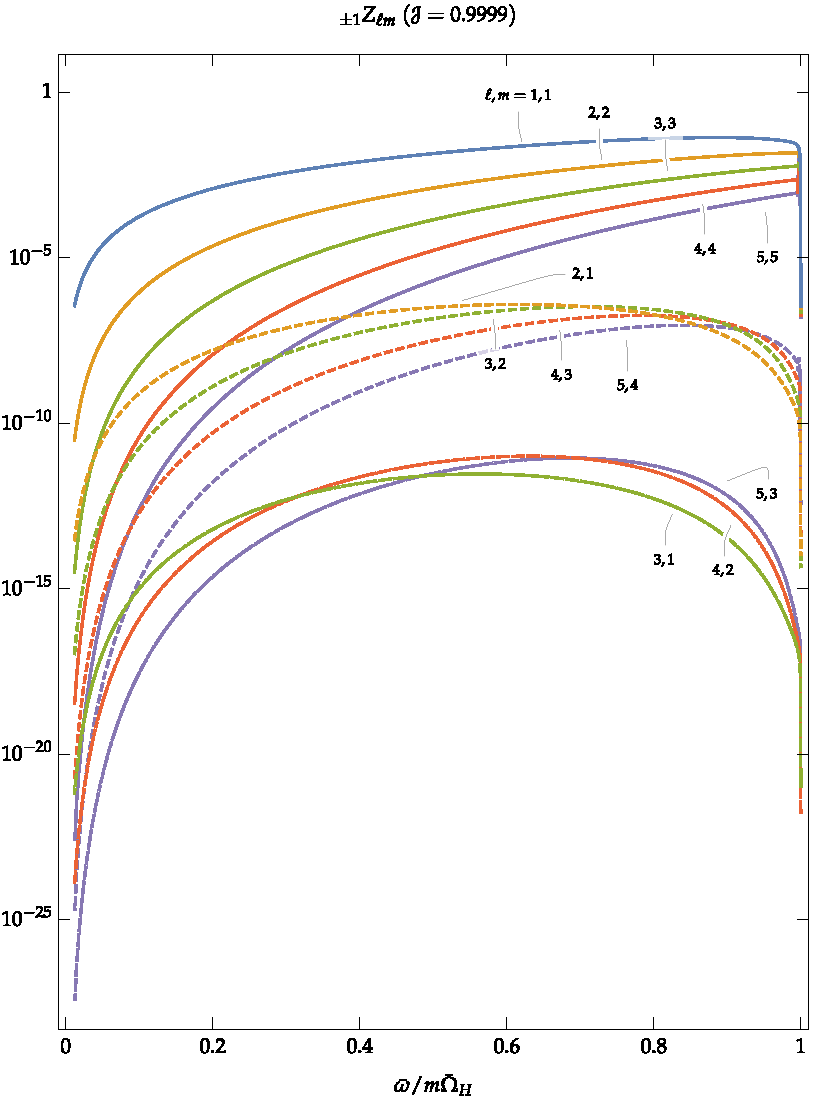
\includegraphics[scale=0.47]{precisionLogZ}
		\end{column}
	\end{columns}
\end{frame}

\begin{frame}[fragile]{Newman-Penrose formalism}
	$\nabla_\mu F^{\mu\nu} = 0 ~,~ \nabla_{[\mu} F_{\nu\rho]} = 0  ~\longrightarrow~$ 4 first-order coupled equations $(\phi_0, \phi_1, \phi_2)$ \\
	$\hspace{1.5cm}\xDownarrow{0.25cm}$
	\metroset{block=fill}
	\begin{alertblock}{Teukolsky's equation}
		\begin{align*}
		& \frac{1}{\Delta^s} \frac{\partial}{\partial r} \left( \Delta^{s+1} \frac{\partial \Upsilon_s}{\partial r} \right) 
		+ \frac{1}{\sin\theta} \frac{\partial}{\partial\theta} \left( \sin\theta \frac{\partial \Upsilon_s}{\partial \theta} \right) 
		- \left[ \frac{(r^2+a^2)^2}{\Delta} - a^2 \sin^2\theta \right]\frac{\partial^2 \Upsilon_s}{\partial t^2} \\[0.15cm]
		& - \frac{4 M a r}{\Delta}\frac{\partial^2 \Upsilon_s}{\partial t \partial \varphi} 
		- \left( \frac{a^2}{\Delta} -\frac{1}{\sin^2\theta} \right)\frac{\partial^2 \Upsilon_s}{\partial \varphi^2} 
		+ 2s\left[ \frac{M(r^2-a^2)}{\Delta} - r - i a \cos\theta \right] \frac{\partial \Upsilon_s}{\partial t} \\[0.15cm]
		&+ 2s\left[ \frac{a(r-M)}{\Delta}+\frac{i \cos\theta}{\sin^2\theta}\right] \frac{\partial \Upsilon_s}{\partial \varphi}
		- (s^2 \cot^2\theta - s) \Upsilon_s = 0 
		\end{align*}
	\end{alertblock}
	
	\begin{center}
		\tabulinesep=0.5mm
		\begin{tabu}{|@{\hskip 0.25cm}c@{\hskip 0.25cm}|c@{\hskip 0.25cm}|}
			\hline
			Spin-weight $s$ & $\Upsilon_s = \int\dd\omega \,\sum_{\ell,m} e^{-i\omega t + i m \varphi} \, {}_{s}S_{\ell m}(\theta) {}_{s}R_{\ell m}(r) $ \\
			\hline\hline
			$+1$ & $\Phi_0 \equiv \phi_0$ \\
			\hline
			$-1$ & $\Phi_2 \equiv 2 (\bar{\rho}^*)^2 \phi_2$ \\
			\hline
		\end{tabu}
	\end{center}
	$\rightarrow$ Describes other perturbations: scalar ($s=0$), GWs ($s=\pm 2$)  
	
\end{frame}


{
\usebackgroundtemplate{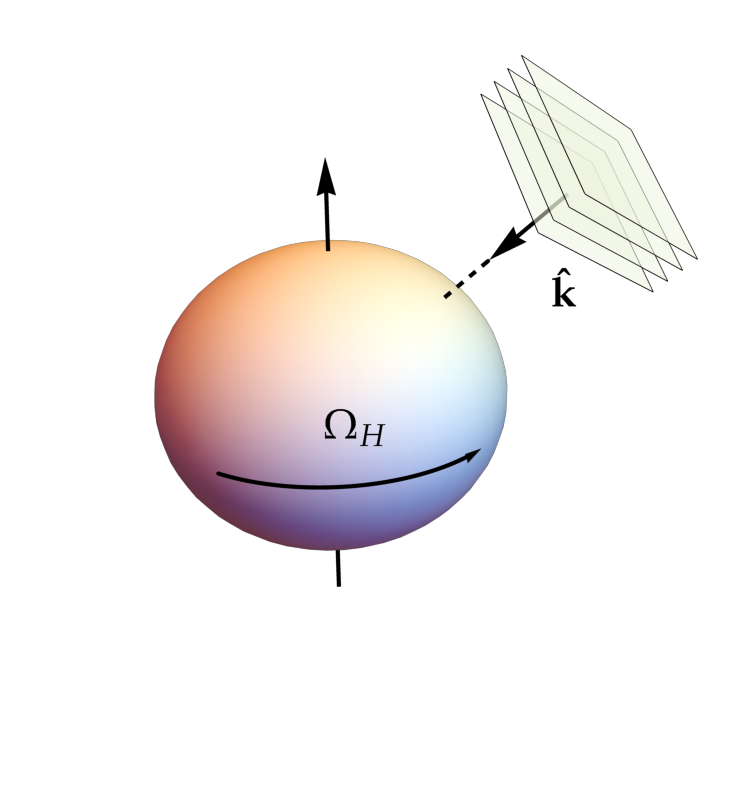
\includegraphics[scale=0.50,trim=-13.5cm 0 0 6]{test.pdf}}
\begin{frame}[fragile]{Scattering of plane waves}
	\begin{columns}[T,onlytextwidth]        
		\begin{column}{0.60\textwidth}
			\begin{itemize}
				\item Astrophysical source: neutron star binary system with magnetic moment
				$$ \mathbf{m}_P = \frac{m_P}{2} \left[ e^{-i \omega t} \sin\alpha_S ( \mathbf{\hat{x}} \pm i \mathbf{\hat{y}}) + \cos\alpha_S \,\mathbf{\hat{z}} \right] $$

				\item Scattering description 
				$$ \phi_2{}^\text{(scatt)} =  \phi_2{}^\text{(pl)} + f(\theta,\varphi) \frac{e^{- i\omega t + i\omega r_*}}{r} $$

				\item Desccription in NP formalism 
				$ \mathbf{m}_P = \frac{m_P}{2} \left[ e^{-i \omega t} \sin\alpha_S ( \mathbf{\hat{x}} \pm i \mathbf{\hat{y}}) + \cos\alpha_S \,\mathbf{\hat{z}} \right] + \text{ c.c.} $
			\end{itemize}
		\end{column}
	\end{columns}
\end{frame}
}

\begin{frame}{Scattering of plane waves}
	\begin{figure}
		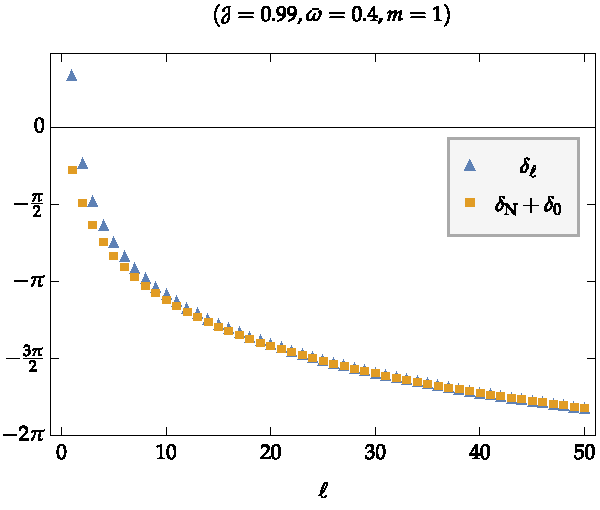
\includegraphics[scale=0.5]{arg2}
		$\Longrightarrow$
		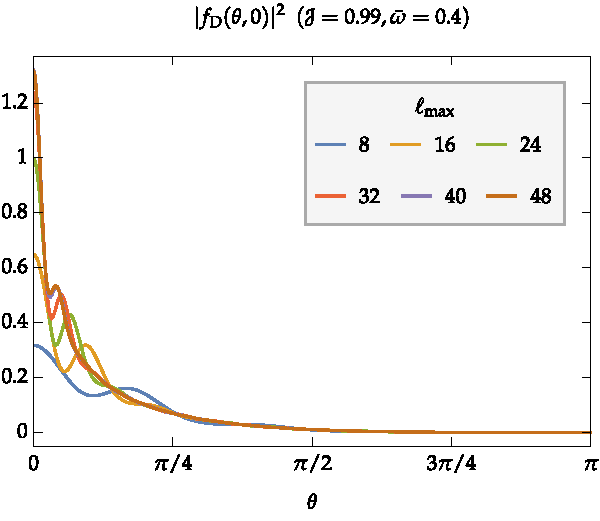
\includegraphics[scale=0.5]{sumFD2}
	\end{figure}
\end{frame}

\begin{frame}{Conclusions / Future work}
	\begin{block}{Conclusions}
		\begin{itemize}
			\item Conclusion 1
			\item Conclusion 2
			\item Conclusion 3
		\end{itemize}
	\end{block}
	\begin{block}{Future work}
		\begin{itemize}
			\item Work 1
			\item Work 2
		\end{itemize}
	\end{block}
\end{frame}

\begin{frame}[standout]
	\huge\textsc{ Questions ? }
\end{frame}

\end{document}